\documentclass[tikz,border=10pt]{standalone}
\usepackage{tkz-euclide} % 引入几何增强包，简化旋转操作

\begin{document}
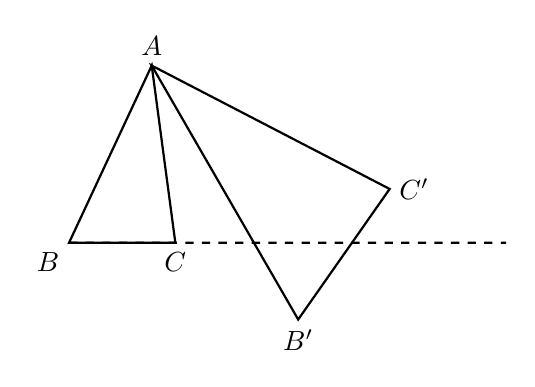
\begin{tikzpicture}[scale=1.5, >=stealth]
    % 1. 定义初始点坐标 (三角形 ABC)
    \coordinate (A) at (1, 2);    % 顶点 A
    \coordinate (B) at (0.3, 0.5); % 顶点 B
    \coordinate (C) at (1.2, 0.5); % 顶点 C

    % 2. 定义旋转参数
    % 设定顺时针旋转角度，例如 -50 度
    \def\rotateAngle{55} 
    \def\scaleFactor{1.5}

    % 3. 计算旋转后的点坐标 (B', C')
    % 以 A 为中心旋转 B 得到 B'
    \path let \p1 = ($(B)-(A)$), \n1 = {atan2(\y1,\x1) + \rotateAngle}, \n2 = {veclen(\x1,\y1) * \scaleFactor}  % 原长度 × 拉长倍数} 
          in coordinate (B1) at ($(A) + (\n1:\n2)$);
    
    % 以 A 为中心旋转 C 得到 C'
    \path let \p1 = ($(C)-(A)$), \n1 = {atan2(\y1,\x1) + \rotateAngle}, \n2 = {veclen(\x1,\y1) * \scaleFactor} 
          in coordinate (C1) at ($(A) + (\n1:\n2)$);

    % 4. 绘制辅助虚线 (经过 BC 并向右延伸)
    \draw[dashed, thick] (B) -- (4, 0.5);

    % 5. 绘制原三角形 ABC
    \draw[thick] (A) -- (B) -- (C) -- cycle;

    % 6. 绘制旋转后的三角形 AB'C'
    \draw[thick] (A) -- (B1) -- (C1) -- cycle;

    % 7. 标注顶点文字
    \node[above] at (A) {$A$};
    \node[below left] at (B) {$B$};
    \node[below] at (C) {$C$};
    \node[below] at (B1) {$B'$};
    \node[right] at (C1) {$C'$};

    % (可选) 绘制旋转弧线以增强表现力
    % \draw[->, bend left] (0.8, 1.8) to node[auto] {} (1.2, 1.8);

\end{tikzpicture}
\end{document}